% !TeX root = HW2_Integrated.tex
% !TeX program = xelatex
\documentclass[11pt]{article}
\usepackage[preprint]{acl}
\usepackage{latexsym}
\usepackage{fontspec}
\usepackage{xeCJK}
\IfFontExistsTF{Times New Roman}{\setmainfont{Times New Roman}}{\setmainfont{TeX Gyre Termes}}
\IfFontExistsTF{Microsoft JhengHei}{\setCJKmainfont{Microsoft JhengHei}}{\setCJKmainfont{Noto Sans CJK TC}}
\usepackage{graphicx,booktabs,amsmath,amssymb,array}
\graphicspath{{../figures/}}
\title{Phishing Website Anomaly Detection:\\Reconstruction Scores, Feature Selection, and Operational Trade-offs}
\author{Team ID: [G01] \\
Seven members' names and student IDs: [515559007馮昱祥、315554053邱育宏、315551146吳宥駒、\\314551160林暉庭、315561001黃少鋒、315561002莊誌強、315554001杜洺鋒] \\
GitHub repository: \url{https://github.com/v1852465cs15/HW2-Anomaly-Detection}}
\raggedbottom
\setlength{\textfloatsep}{10pt plus 2pt minus 2pt}
\setlength{\dbltextfloatsep}{10pt plus 2pt minus 2pt}
\setlength{\floatsep}{8pt plus 2pt minus 2pt}
\setlength{\dblfloatsep}{8pt plus 2pt minus 2pt}
\setlength{\intextsep}{8pt plus 2pt minus 2pt}
\setlength{\abovecaptionskip}{4pt}
\begin{document}
\maketitle
\begin{abstract}
Phishing alerts must protect users without overwhelming analysts. On 11,055 tabular records, a normal-only categorical AE achieves five-seed AP .940, exceeding heuristic/Isolation Forest baselines but trailing supervised XGBoost (.998). Top-9 MI features retain close performance; redundancy conclusions depend on the cutoff. Training contamination of 10\% reduces AP from .939 to .709. Additive explanations and six failure cases expose legitimate-like phishing and rare benign profiles. At 1\% prevalence, FPR constraints reduce projected false alarms from 701 to 99 per 10,000 scans at lower recall. Duplicate vectors and untested distribution shift limit deployment claims.
\end{abstract}
\section{Introduction}
We study \textbf{Tabular} phishing detection with 30 categorical indicators, without URLs/HTML. A feature-wise softmax AE models code combinations without numeric-distance assumptions. Legitimate \texttt{train\_00000} has (SSL, anchor)=$(1,1)$; phishing \texttt{train\_00002} has $(-1,-1)$: coded examples, not live inspections.

Security analysts review alerts, warn users, and block confirmed threats. FPs waste review capacity/disrupt visits; FNs expose users to credential theft.

\textbf{Research question:} Can normal-only reconstruction detect phishing while preserving performance with nine features and controlling false-alarm workload?

Our contributions are:

\textbf{(1)} a shared-split three-tier comparison with explicit supervision differences.

\textbf{(2)} training-only MI/redundancy evidence and controlled feature, contamination, and scoring ablations.

\textbf{(3)} score-level explanations, concrete FP/FN cases, and prevalence-adjusted workload estimates.

\section{Related Work}
Our category is \textbf{Tabular}; the following studies differ in data, method, supervision, and outcomes.

\citet{hannousse2021}: 87 URL/content/service features, supervised Random Forest, accuracy 96.61\% hybrid/96.83\% after selection. We instead test normal-only fitting and redundancy on 30 tabular codes.

\citet{bu2021}: 222,541 URLs, three corpora, character-level convolutional AE plus supervised auxiliary CNN; reported sensitivity gain 3.98\%. We reconstruct tabular codes with additive explanations.

\citet{sahingoz2019}: 73,575 URLs, supervised Random Forest/NLP, accuracy 97.98\%. We compare supervision and alert costs; cross-dataset scores are contextual.

Tier assumptions: $-1$ counts reflect risk (Tier 1 floor); normal combinations reconstruct well or anomalies isolate easily (Tier 2 AE/Isolation Forest; \citet{liu2008}); labeled phishing generalizes (Tier 3 XGBoost; \citet{chen2016}).
\section{Task Definition \& Data}
We use UCI Phishing Websites: 11,055 records, 30 categorical features, sourced from PhishTank, MillerSmiles, and Google search operators \citep{uci}. Inherited labels define legitimate ($Result=1,y=0$) versus phishing ($Result=-1,y=1$). Anomaly means phishing, not rarity: 4,898 (44.31\%) phishing and 6,157 (55.69\%) legitimate, approximately $1:1.26$.

Always-normal achieves 55.69\% accuracy but misses every phishing site. This moderate imbalance and deployment-prevalence mismatch motivate AP, recall, FPR, and workload projections at 1\% prevalence rather than accuracy.

\begin{table}[t]\centering\small
\begin{tabular}{lrrr}\toprule
Partition & Total & Legitimate & Phishing\\\midrule
Training & 7,738 & 4,310 & 3,428\\
Validation & 1,658 & 923 & 735\\
Test & 1,659 & 924 & 735\\\bottomrule
\end{tabular}
\caption{Our stratified split; one-class models fit the legitimate training subset only.}\label{tab:data}
\end{table}
The 70/15/15 split retains 5,206 extra duplicate labeled rows, 5,270 extra feature vectors, and 64 conflicting-label groups, suggesting representation ambiguity or annotation noise. No features are missing/constant. URL, HTML, form, and reputation indicators are categorical; zero is not missingness.

\section{Exploratory Feature Analysis}
\textbf{Mutual Information Ranking.} Higher MI indicates more information about legitimate versus phishing labels. We compute MI in nats on 7,738 training records only; this label-assisted selection is separate from normal-only AE fitting. Figure~\ref{fig:training}(a) ranks all features. The Top-9 are SSLfinal\_State, URL\_of\_Anchor, Prefix\_Suffix, web\_traffic, having\_Sub\_Domain, Links\_in\_tags, Request\_URL, SFH, and Domain\_registeration\_length.

The exploratory cutoff follows MI's 3.43-fold drop from rank 9 (.02461) to 10 (.00717), motivating 70\% feature reduction with Top-5/15 controls. It is not uniquely optimal; lower-MI features may remain useful.

\textbf{Normal versus phishing.} Figure~\ref{fig:training}(c): SSL code $1$ is 89.12\% legitimate; $-1$ is 85.74\% phishing. In (d), anchor code $-1$ is 99.00\% phishing; $1$ is 94.15\% legitimate. These within-code class shares show overlap; neither feature determines the label.

\textbf{Feature Association.} Higher Cramer's V in Figure~\ref{fig:training}(b) suggests overlapping information. We use training-only Pearson counts, $V=\sqrt{\chi^2/[n\min(r-1,c-1)]}$, without Yates correction. The exploratory cutoff $V\geq.80$ was not preregistered.

\begin{table}[h]\centering\small
\begin{tabular}{lrrrr}\toprule
Features & Pairs & $V\geq.50$ & $V\geq.80$ & Max $V$\\\midrule
All 30 & 435 & 25 & 4 & .939\\
Top 9 & 36 & 1 & 0 & .606\\\bottomrule
\end{tabular}
\caption{Training-only pairwise redundancy sensitivity ($n=7,738$); diagonal and mirrored pairs are excluded.}\label{tab:v}
\end{table}
Four pairs reach $V\geq.80$: Favicon/popUpWidnow (.9394), URL shortener/double-slash redirect (.8405), Favicon/port (.8027), and port/email submission (.8008); Figure~\ref{fig:training}(b) gives feature codes. Top-9's maximum, registration length/Request\_URL (.6057), exceeds .50/.60. Redundancy is cutoff-dependent; pairwise V cannot establish conditional complementarity.

\textbf{H1:} Selecting the top 9 features based on Mutual Information can achieve comparable anomaly detection performance to using all 30 features.

\textbf{H2:} The top 9 features provide sufficient complementary information for phishing website detection without highly redundant features.

\begin{figure*}[t]\centering
\begin{minipage}[t]{.48\textwidth}\centering (a) MI ranking\\
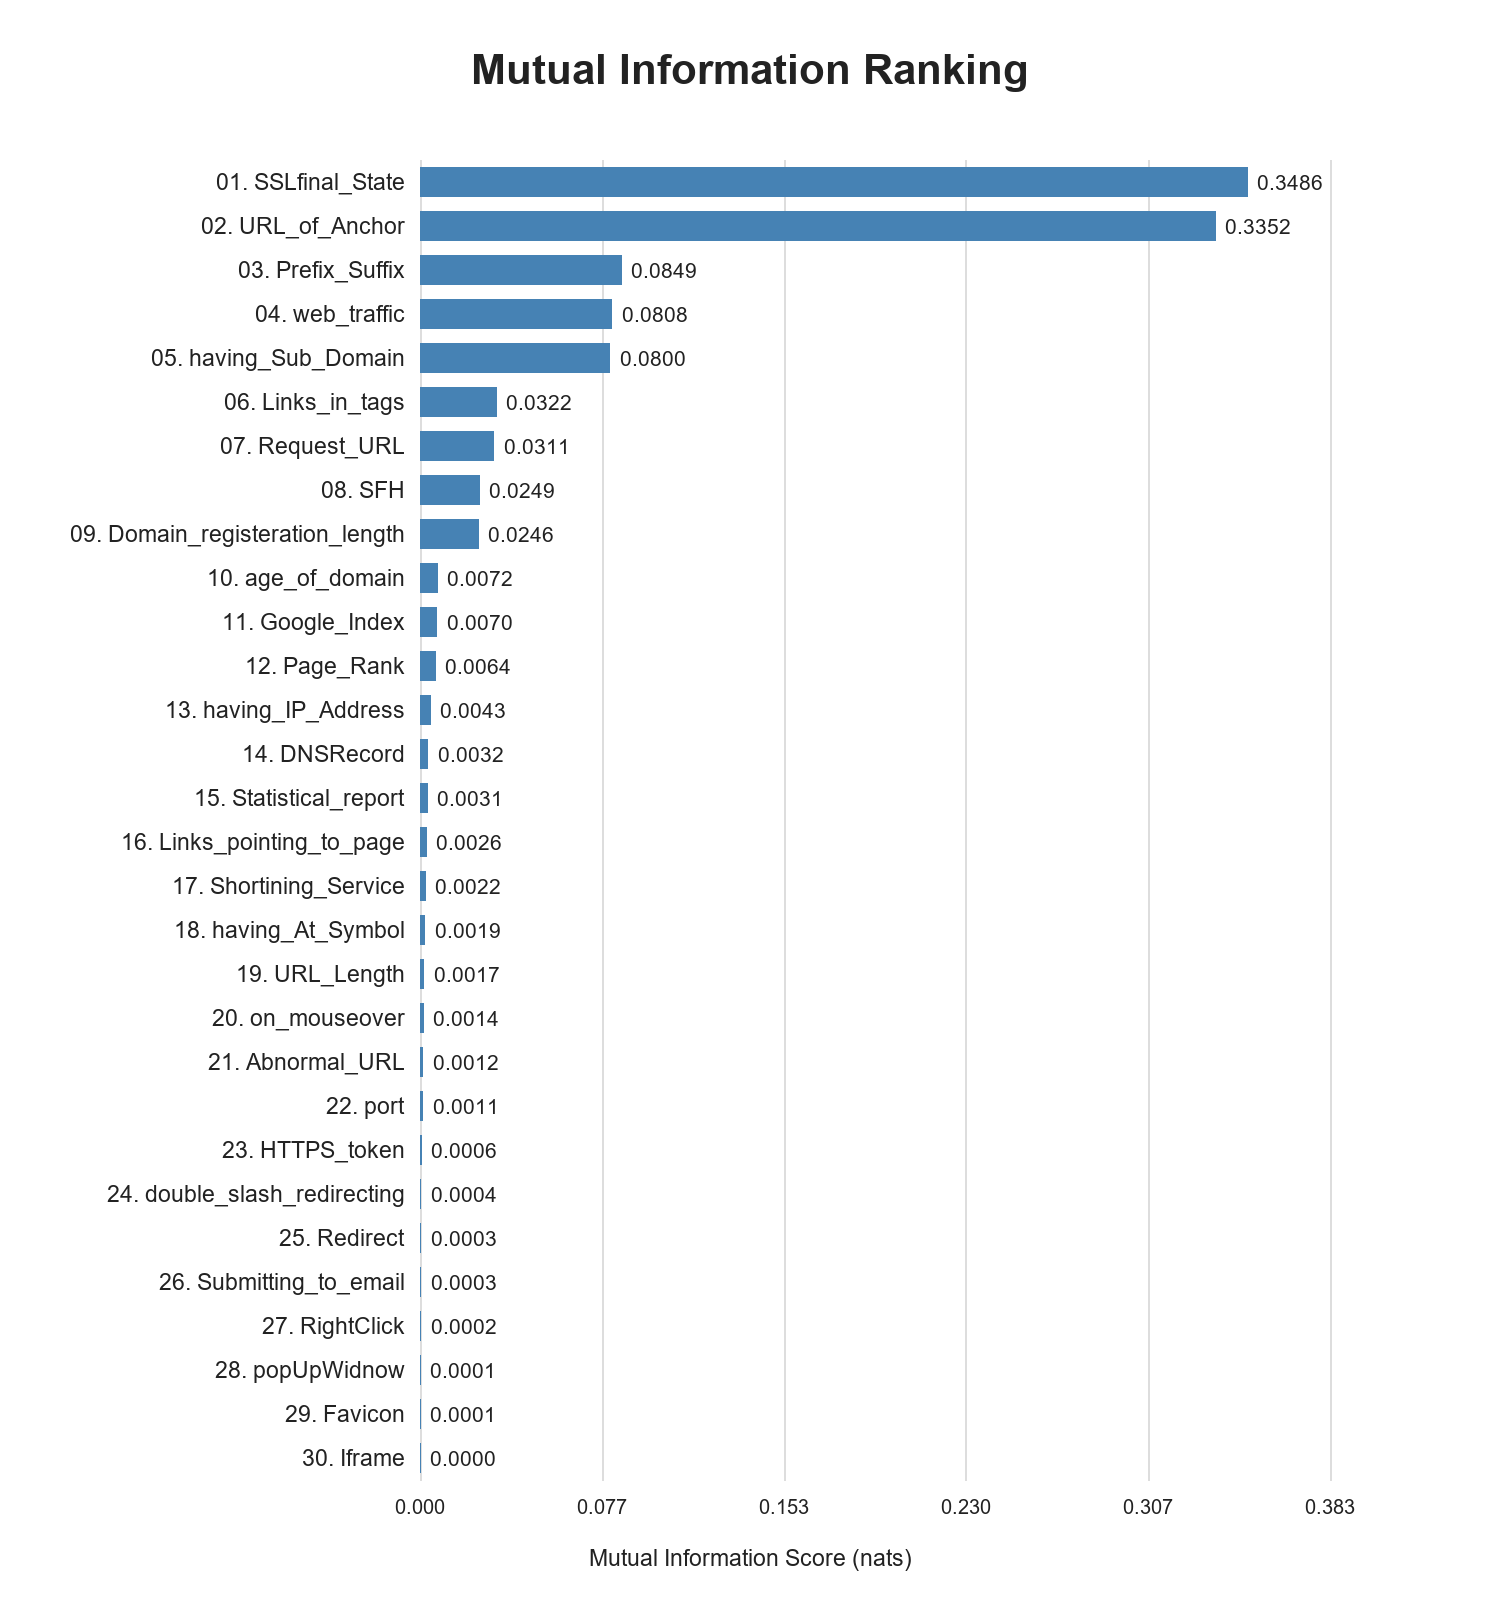
\includegraphics[width=\linewidth]{A_figures/MI_Ranking.png}\end{minipage}\hfill
\begin{minipage}[t]{.48\textwidth}\centering (b) Feature association\\
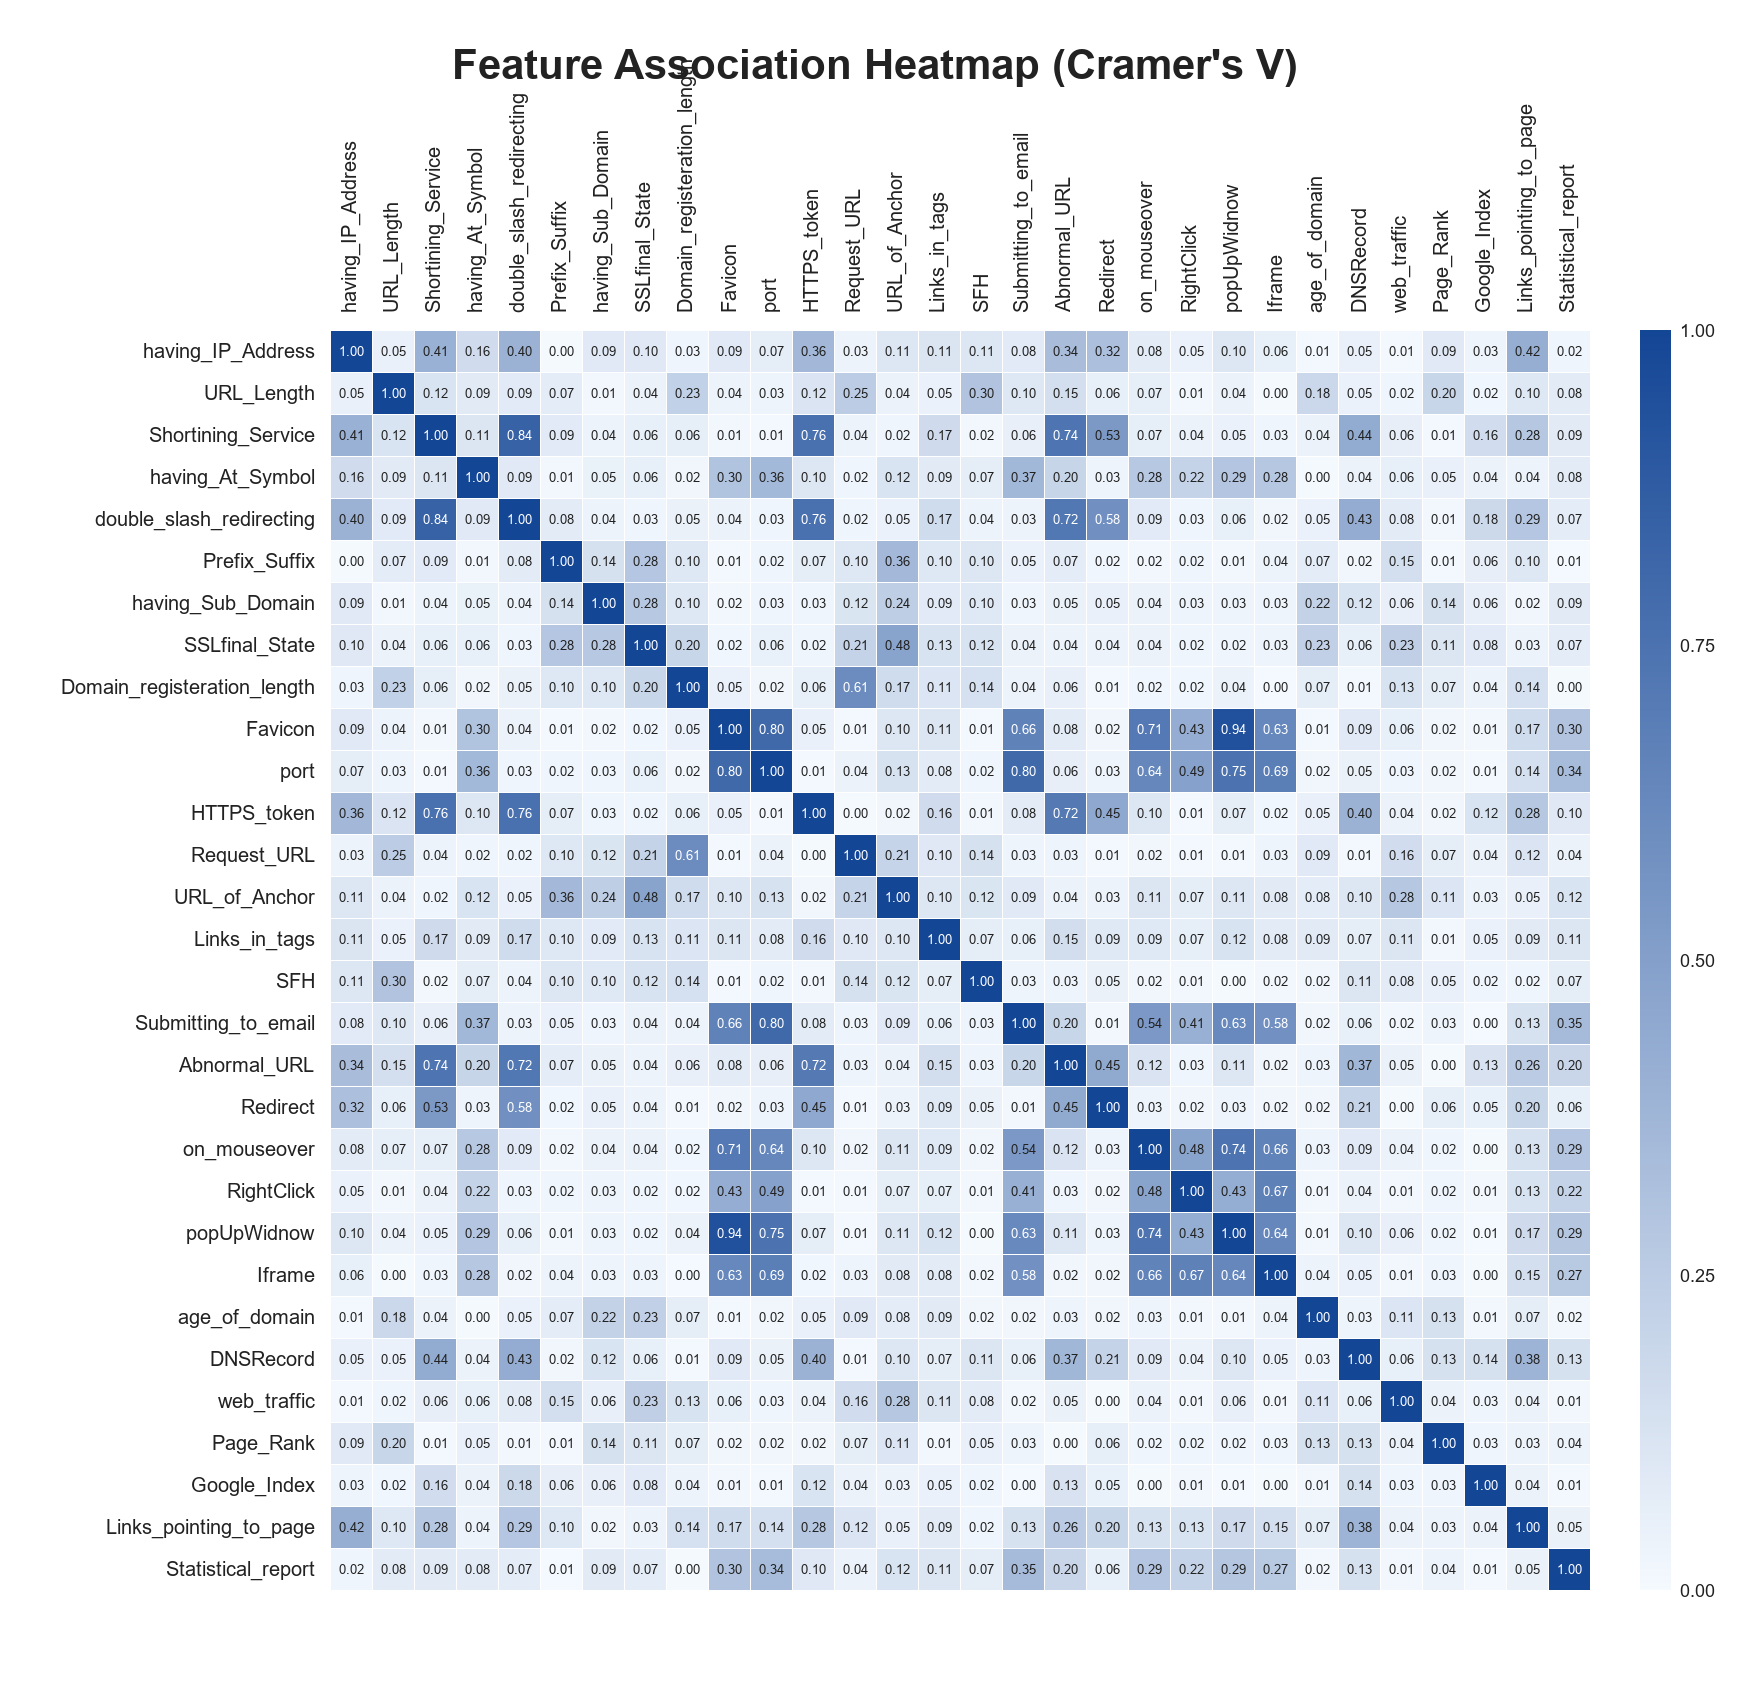
\includegraphics[width=\linewidth]{A_figures/Feature_Association.png}\end{minipage}
\caption{Training-only feature analysis. (a) MI ranking and (b) Cramer's V heatmap with feature names and numerical annotations. Class-conditional evidence is continued in (c)--(d).}\label{fig:training}
\end{figure*}
\begin{figure*}[t]\centering
\begin{minipage}[t]{.48\textwidth}\raggedright (c) SSL-state distribution\\
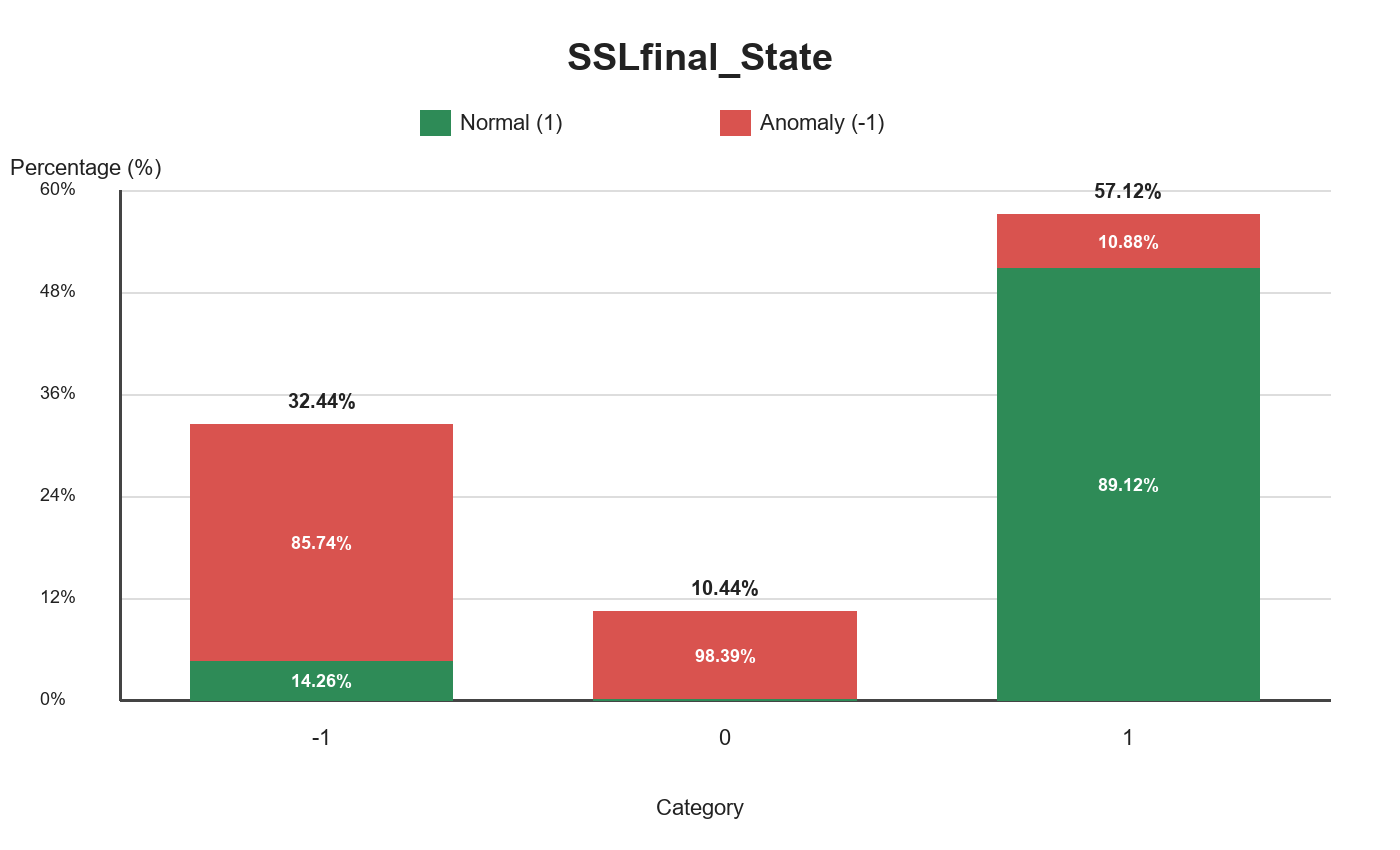
\includegraphics[width=\linewidth]{A_figures/Feature_Abnormal_Distribution/SSLfinal_State.png}\end{minipage}\hfill
\begin{minipage}[t]{.48\textwidth}\raggedright (d) Anchor-code distribution\\
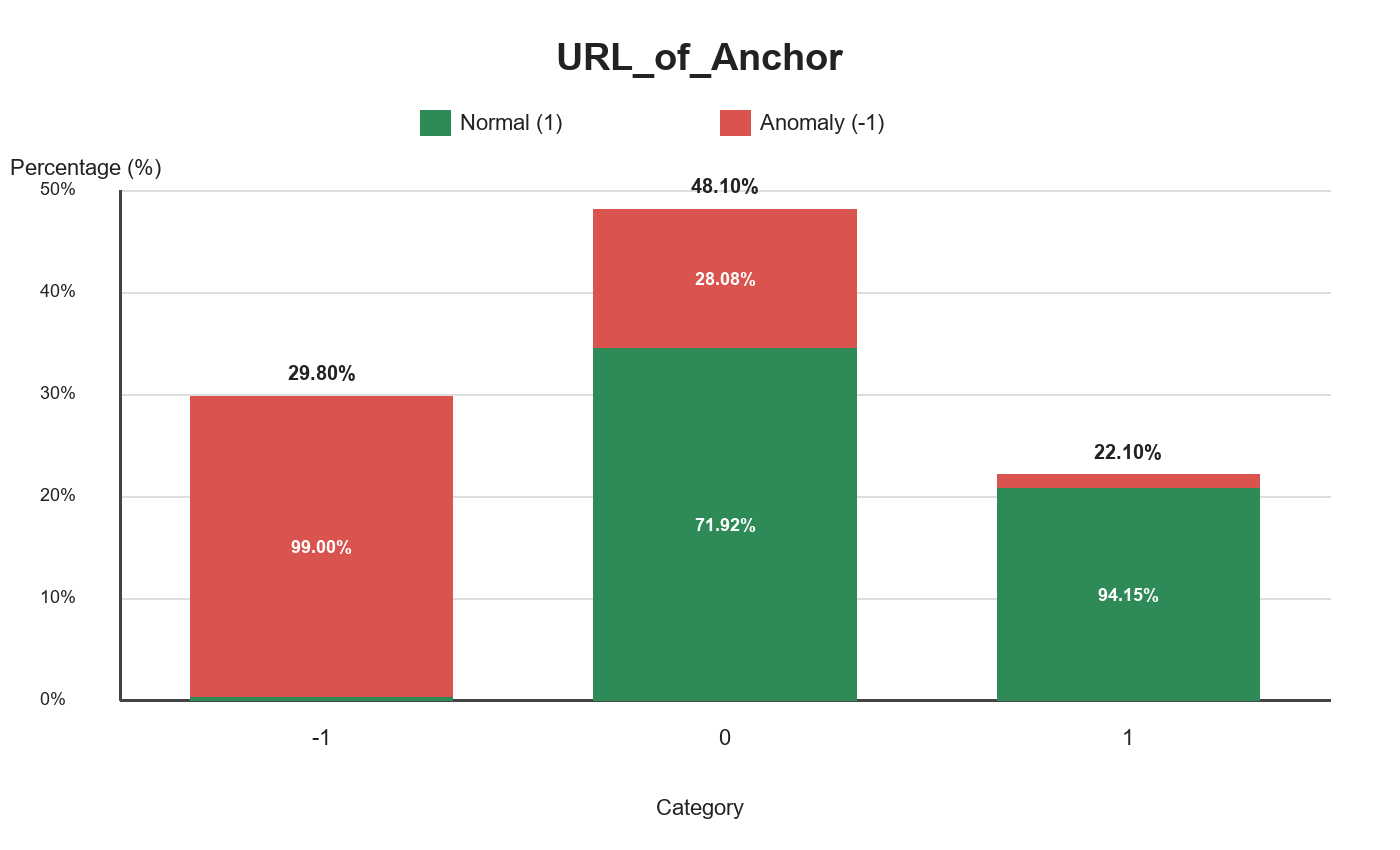
\includegraphics[width=\linewidth]{A_figures/Feature_Abnormal_Distribution/URL_of_Anchor.png}\end{minipage}
\addtocounter{figure}{-1}
\caption{(continued) (c)--(d): bar heights are category shares of training records; labels within bars are within-category class shares.}
\end{figure*}
\section{Method}
\subsection{Categorical reconstruction}
Three-position one-hot encoding gives 90 inputs without fitted vocabularies/scalers. The AE is $90\rightarrow128\rightarrow64\rightarrow8\rightarrow64\rightarrow128\rightarrow90$, with feature-wise softmaxes (Figure~\ref{fig:pipeline}); categorical CE fits only 4,310 legitimate training records.

\begin{equation}
\begin{aligned}
s(x)&=\sum_{j=1}^{30}s_j(x),\\[6pt]
s_j(x)&=-\log\widehat p_j(x_j\mid e(x)).
\end{aligned}
\end{equation}
Larger scores indicate reconstruction surprise; additive feature terms explain the total in nats.
\begin{figure*}[t]\centering
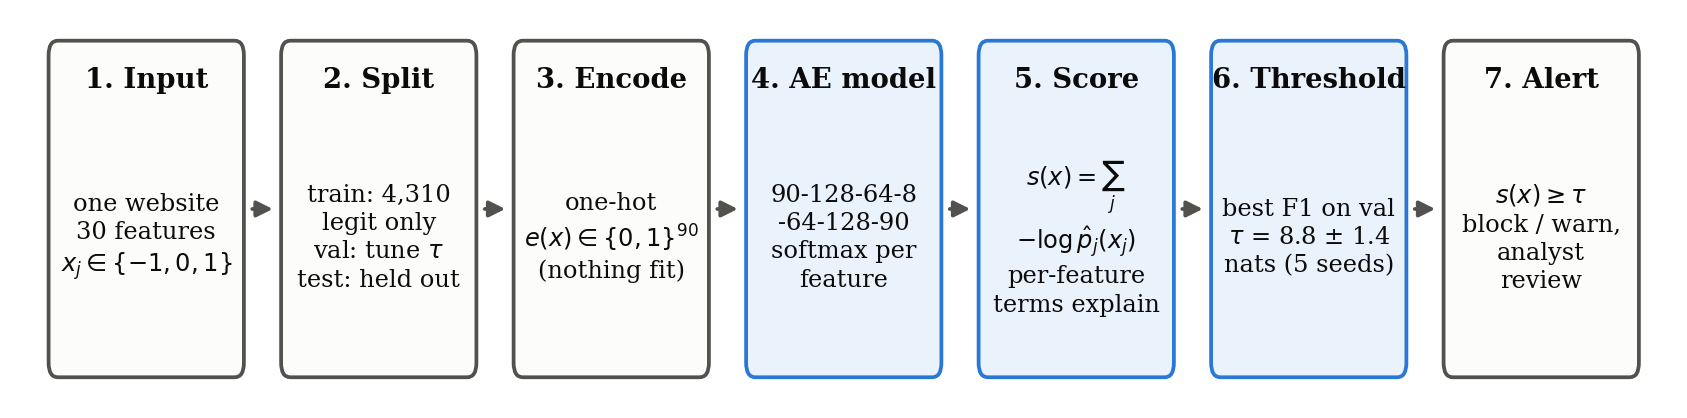
\includegraphics[width=.88\textwidth]{fig_pipeline.png}
\caption{Our categorical AE pipeline. Threshold summary spans five seeds; we fit parameters on legitimate training records only.}\label{fig:pipeline}
\end{figure*}
\subsection{Threshold decision and error costs}
Alert when $s(x)\geq\tau$. Validation-F1 optima are 6.696, 9.230, 8.804, 10.531, 8.691 nats across five seeds (mean 8.79). F1 balances precision/recall but specifies no monetary FP/FN costs and may exceed review capacity at low prevalence.

Alternatively, constrain legitimate-validation FPR to 1\%: suppress costly false warnings/reviews while accepting more FNs. Test FPR is measured separately, not guaranteed. Neither threshold rule uses test labels.

\subsection{Comparison methods}
Tier 1: always-normal and count of $-1$ codes (validation threshold 7), intentionally naive because signs have feature-specific meanings. Normal-only Isolation Forest: 300 trees, 1,024 max samples, .5 max features. Supervised XGBoost: both classes, 500 trees, depth 9, learning rate .05; phishing probability is its score, with a label advantage.

\section{Experimental Setup}
All methods share partitions and seeds 0--4; seeds alter models, not data. Labels/IDs are excluded. Legitimate validation supports early stopping; labeled validation selects parameters/thresholds. AE: Adam ($10^{-3}$), batch 128, maximum 200 epochs, patience 10.

Validation grids cover AE hidden layers $(64,32)/(128,64)$ and latent widths $\{2,4,8,16\}$; IF trees $\{100,300\}$, samples $\{256,1024\}$, feature fractions $\{.5,1\}$; XGBoost trees $\{200,500\}$, depths $\{3,6,9\}$, rates $\{.05,.1\}$. We use PyTorch 2.7.1, scikit-learn 1.6.1, XGBoost 3.0.1, and SciPy 1.15.2 on an AMD Ryzen 5 5600H CPU, no GPU.

Metrics: AP (average precision, not trapezoidal PR-AUC), ROC-AUC, F1, recall, and $FPR=FP/(FP+TN)$. We report five-seed means/SDs, paired seed-wise $t$-tests, and 2,000 paired site bootstraps of seed-averaged scores.

\textbf{Overlap limitation:} 987/1,659 test rows share training vectors (829 distinct); 672 are unseen. The split is not group-disjoint; unseen-vector results are sensitivity checks. Site bootstraps ignore vector-cluster dependence, limiting generalization claims.
\section{Results}
\subsection{Main comparison}
AE exceeds heuristic/IF but trails supervised XGBoost (Table~\ref{tab:main}; Figure~\ref{fig:pr}). Versus IF, AP gap is $+.2919$ (95\% bootstrap CI $[.2583,.3232]$, paired $p=1.03\times10^{-6}$); versus XGBoost, $-.0498$ ($[-.0592,-.0401]$, $p=1.78\times10^{-6}$). Gaps use AP of seed-averaged scores; Table~\ref{tab:main} averages per-seed AP. Nonlinearity explains its different differences ($+.283/-.058$).
\begin{table*}[t]\centering\small
\begin{tabular}{llrrrrrr}\toprule
Tier & Method & AP & ROC-AUC & F1 & FPR $\downarrow$ & AP unseen & Train s / ms site\\\midrule
1 & Always normal & .443$\pm$.000 & .500$\pm$.000 & .000$\pm$.000 & .000$\pm$.000 & .567$\pm$.000 & 0 / $<$.001\\
1 & Count of $-1$ & .625$\pm$.000 & .710$\pm$.000 & .706$\pm$.000 & .562$\pm$.000 & .690$\pm$.000 & 0 / $<$.001\\
2 alt. & Isolation Forest & .657$\pm$.014 & .724$\pm$.013 & .690$\pm$.010 & .548$\pm$.020 & .728$\pm$.009 & .42 / .029\\
2 & Autoencoder & .940$\pm$.003 & .933$\pm$.003 & .856$\pm$.009 & .071$\pm$.017 & .943$\pm$.004 & 8.41 / .002\\
3 & XGBoost & \textbf{.998$\pm$.000} & \textbf{.998$\pm$.000} & \textbf{.973$\pm$.001} & .029$\pm$.001 & \textbf{.998$\pm$.000} & .47 / .003\\\bottomrule
\end{tabular}
\caption{Our test results, mean $\pm$ SD over five seeds; unseen-vector $n=672$. AP denotes average precision. Latency excludes feature extraction; zero rounded SD is not exact equality.}\label{tab:main}
\end{table*}\begin{figure}[t]\centering
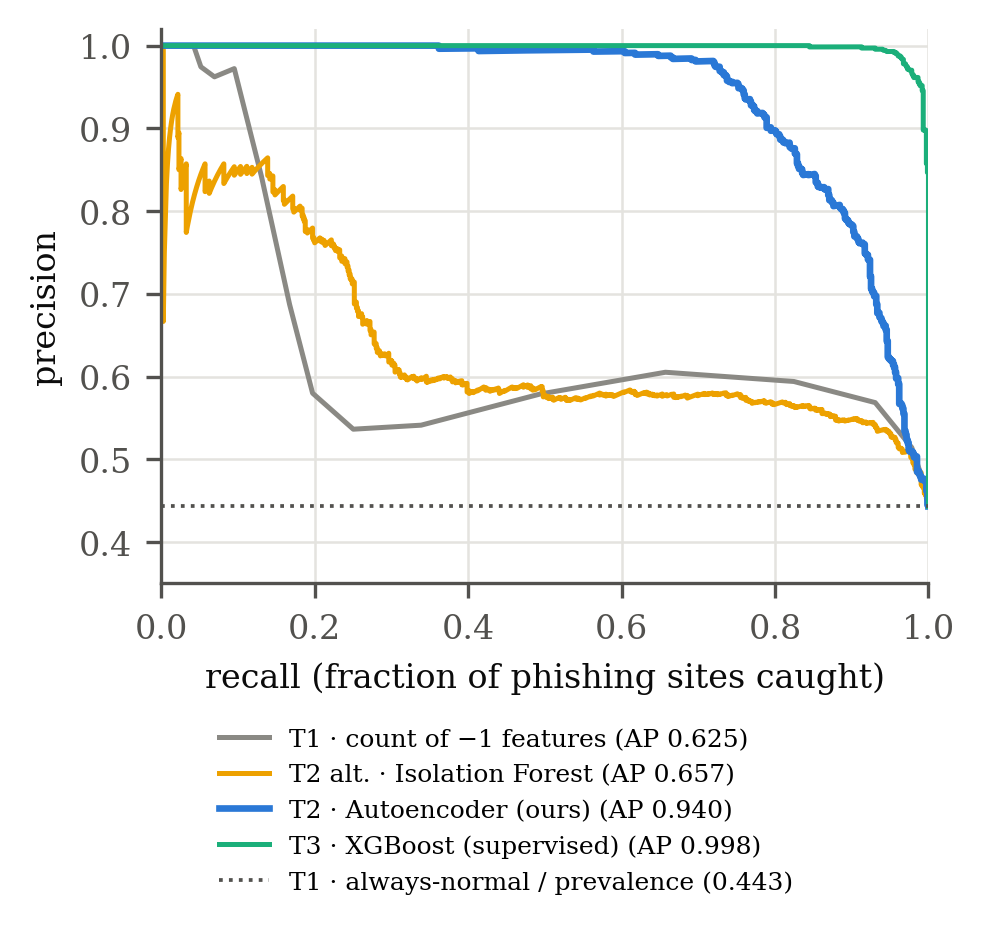
\includegraphics[width=\columnwidth]{fig_pr_curves.png}
\caption{Our seed-0 test PR curves. The dotted line is a constant-score AP reference, not operational precision of a no-alert detector.}\label{fig:pr}
\end{figure}\begin{figure}[t]\centering
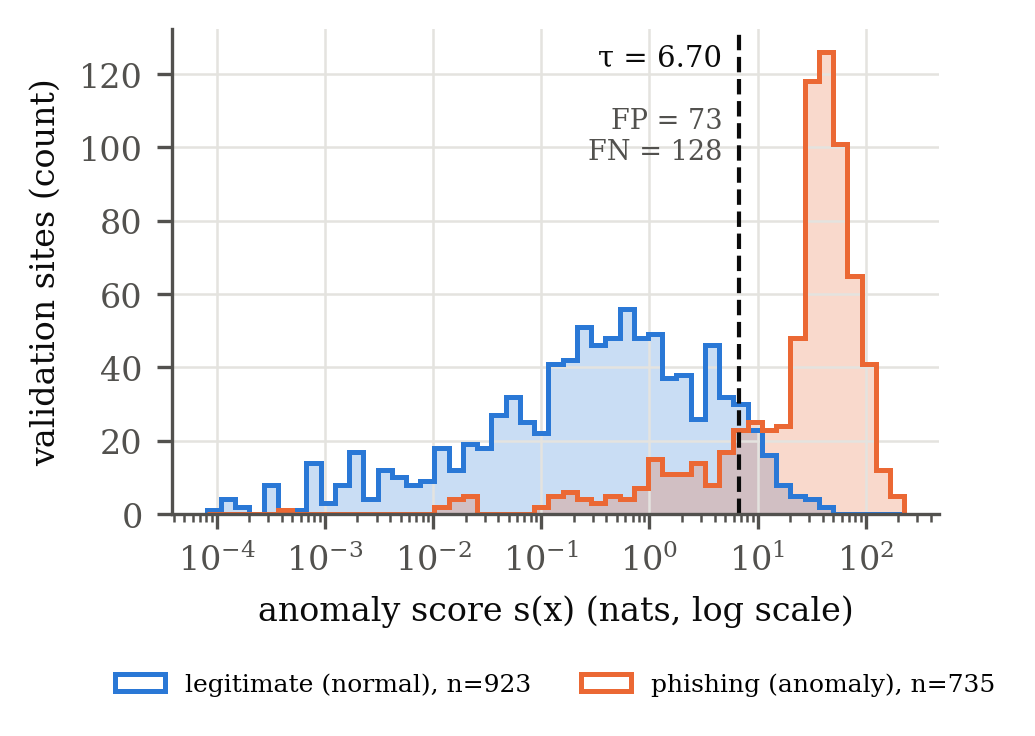
\includegraphics[width=\columnwidth]{fig_score_dist.png}
\caption{Our seed-0 validation scores and $\tau=6.70$ nats. FP=73/FN=128 are validation counts; test counts are FP=92/FN=126.}\label{fig:scores}
\end{figure}
Unseen-vector AP is .943 (AE) versus .998 (XGBoost), with prevalence .567 rather than .443; overlap is not thereby harmless. Figure~\ref{fig:scores} shows below-threshold phishing. AE takes 8.41 s to train and .002 ms/site in batch, excluding feature extraction: stronger ranking than IF at higher training cost, but weaker than supervised XGBoost.

\subsection{Controlled ablations}\label{sec:ablation}
Ablations hold split, seeds and validation-F1 selection fixed. Their baseline AP/F1 .939/.851 differs from main-run .940/.856 by .001/.005, within one seed SD (.003/.009); separate run sets do not imply identical conditions.

Top-9 AP is $.933\pm.010$ (gap $-.0063$, $p=.242$), F1 .854: descriptive H1 support, not preregistered equivalence. Top-15 AP .951 means nine is not proven optimal (Table~\ref{tab:abl}).
\begin{table}[t]\centering\small
\begin{tabular}{lrrr}\toprule
Configuration & AP $\pm$ SD & F1 & $p$ vs. full\\\midrule
Full 30 / clean / CE & .939$\pm$.003 & .851 & --\\
Top 5 & .932$\pm$.011 & .862 & .304\\
Top 9 (H1/H2) & .933$\pm$.010 & .854 & .242\\
Top 15 & .951$\pm$.004 & .873 & .0216\\
Contamination 1\% & .865$\pm$.011 & .802 & .000168\\
Contamination 5\% & .779$\pm$.019 & .748 & .0000262\\
Contamination 10\% & .709$\pm$.018 & .693 & .0000131\\
MSE scoring & .914$\pm$.003 & .835 & .000504\\\bottomrule
\end{tabular}
\caption{Our controlled ablations across five seeds. Uncorrected paired $t$-test $p$ values; Bonferroni criterion $\alpha=.05/7\approx.00714$ for seven comparisons.}\label{tab:abl}
\end{table}
H2 has partial support: zero Top-9 pairs at $V\geq.80$, one at $.50$ (Table~\ref{tab:v}). Close AP supports useful combined information, not conditional complementarity/minimality; leave-one-feature-out tests remain necessary.

With $n=4,310$, 1/5/10\% contamination lowers AP to .865/.779/.709; 10\% raises FPR from 7.5\% to 48.1\%. CE training/MSE scoring gives AP .914, FPR 14.0\%. These effects survive Bonferroni ($\alpha=.05/7\approx.00714$), unlike Top-15 ($p=.0216$). Clean data and categorical scoring matter most.

\section{Analysis}
\subsection{Error Analysis}
At $\tau=6.696$ nats, seed 0 yields 126 FNs/92 FPs on 1,659 test sites (TP=609, TN=832; Table~\ref{tab:breakdown}). Near misses satisfy $.5\leq s/\tau\leq2$; inversions are at least tenfold off. Hamming distance uses the nearest legitimate training site. Conflicts suggest label noise or lossy representation; static codes have no sensor noise.

\begin{table}[h]\centering\small\fontsize{10}{11.5}\selectfont
\setlength{\tabcolsep}{2pt}
\renewcommand{\arraystretch}{1.08}
\begin{tabular*}{\columnwidth}{@{\extracolsep{\fill}}>{\raggedright\arraybackslash}p{.44\columnwidth}rr@{}}\toprule
Property & FN ($n=126$) & FP ($n=92$)\\\midrule
Near miss (within $2\times$) & 46 (37\%) & 61 (66\%)\\
Complete inversion ($\geq10\times$) & 39 (31\%) & 0 (0\%)\\
Median $s/\tau$ & .34 & 1.62\\
$\leq1$ code from legit. training & 71 (56\%) & 46 (50\%)\\
Identical vector: both labels & 17 (13\%) & 0 (0\%)\\
Wrong in all five seeds & 86 (68\%) & 13 (14\%)\\
XGBoost correct & 115 (91\%) & 86 (93\%)\\\bottomrule
\end{tabular*}
\caption{Breakdown of all 218 seed-0 test errors.}\label{tab:breakdown}
\end{table}

Table~\ref{tab:errors} selects the lowest-score conflicting FN, lowest-score systematic unseen-vector FN, highest-score FN, lowest/highest-score FP, and systematic FP with a legitimate training vector. Figure~\ref{fig:errors}(a)--(c) shows five score orders among FNs, near-threshold FPs, and weak negative-code signals in missed phishing. First fixes are richer features/limited labels for FNs and FPR constraints/tested score caps for FPs; threshold changes cannot rescue near-zero-score phishing.

\begin{table*}[t]\centering\small
\begin{tabular}{cllrrrrrll}\toprule
\# & Type & Site & SSL & A & T & L & $s(x)$ & $s/\tau$ & Cause\\\midrule
1 & FN & test\_01368 & +1 & 0 & +1 & -1 & .0002 & Inversion ($3\times10^{-5}$) & Label conflict\\
2 & FN & test\_01163 & +1 & 0 & +1 & 0 & .0056 & Inversion ($8\times10^{-4}$) & Missing information\\
3 & FN & test\_01618 & -1 & 0 & +1 & +1 & 6.32 & Near (.94) & Overlap\\
4 & FP & test\_01277 & +1 & +1 & 0 & +1 & 6.73 & Near (1.01) & Overlap\\
5 & FP & test\_01494 & -1 & 0 & +1 & -1 & 44.3 & Far (6.6) & Contextual mismatch\\
6 & FP & test\_00052 & +1 & +1 & -1 & 0 & 13.6 & Far (2.0) & Overlap\\\midrule
\multicolumn{3}{l}{Legitimate training mode} & +1 & 0 & +1 & 0 & & & \\
\multicolumn{3}{l}{Phishing training mode} & -1 & -1 & 0 & -1 & & & \\\bottomrule
\end{tabular}
\caption{Six cases, $\tau=6.696$ nats. A=URL\_of\_Anchor; T=web\_traffic; L=Links\_in\_tags; SSL=SSLfinal\_State. Scores/ratios are rounded; case 6 is just above $2\times$. Signs have feature-specific meanings.}\label{tab:errors}
\end{table*}

\paragraph{Case notes.} (1) Training vector: five legitimate/four phishing; all $s_j\approx0$, XGBoost $P=.50$. (2) Legitimate-like codes; all $s_j\approx0$, $P=.03$. (3) SSL $-1$ contributes 3.60 nats; score is .38 below $\tau$, $P=.73$. (4) Benign deviations add up: Traffic $0$ (1.92), on\_mouseover $-1$ (1.80), Abnormal\_URL $-1$ (1.21). (5) Rare legitimate SSL $-1$ contributes 20.2 (46\%); contextual mismatch does not establish temporal drift. (6) Vector occurs twice as legitimate in training; SFH $+1$ contributes 8.6 (63\%), and all five seeds flag it. Feature terms sum to the total score.

\begin{figure*}[t]\centering
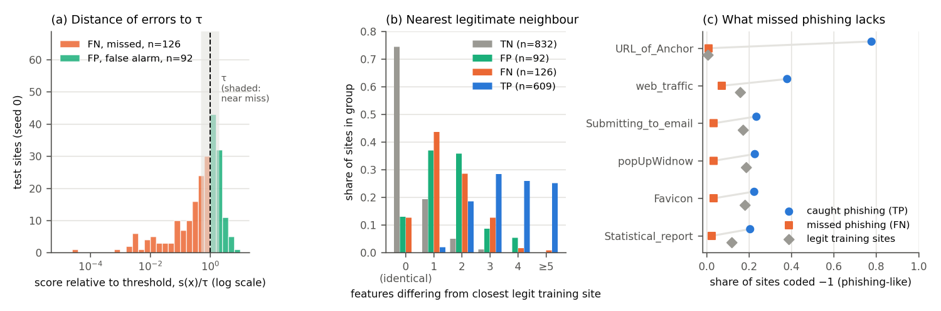
\includegraphics[width=.92\textwidth]{C_figures/fig_error_analysis.png}
\caption{Seed-0 test error analysis: (a) scores relative to $\tau$ (log scale); (b) nearest legitimate-training Hamming distance by outcome; (c) negative-code shares for six features distinguishing caught from missed phishing.}\label{fig:errors}
\end{figure*}

\subsection{Interpretability and faithfulness}
For alert \texttt{test\_00505} ($s=40.2$, $\tau=6.696$), anchor/SSL/tag-link terms are 26.0/7.4/5.6 nats (97\%). Mean anchor/SSL shares are 35\%/17\%. AE rankings correlate with XGBoost mean absolute SHAP \citep{lundberg2020} ($\rho=.81$) and training MI (.83); agreement does not establish causation.

Resetting top 1/2/5 score-driving features to legitimate modes clears 30/54/70\% of 609 true alerts, versus 2\%/9\% for one/five random features (20 repeats). This supports score sensitivity, but edited combinations may be implausible. Explanations support review of coded evidence, not raw pages or near-zero-score attacks.
\subsection{Practical impact}
At 1\% phishing prevalence, 10,000 scans contain 100 phishing/9,900 legitimate sites (Table~\ref{tab:ops}). Holding conditional error rates fixed, FPR constraints raise projected precision from .10 to .41 at 11 extra misses per 100 phishing sites; these are not deployment measurements.
\begin{table}[h]\centering\small
\setlength{\tabcolsep}{3pt}
\begin{tabular}{@{}lrrr@{}}\toprule
AE threshold rule & Caught & Missed & False alerts\\\midrule
Validation best F1 & 81 & 19 & 701\\
Validation FPR $\leq1\%$ & 70 & 30 & 99\\\bottomrule
\end{tabular}
\caption{Our projected counts per 10,000 scans at 1\% phishing prevalence, holding conditional error rates fixed.}\label{tab:ops}
\end{table}
\section{Conclusion \& Limitations}
\subsection{Key decisions, redesign, and future work}
Clean normal-only training was our key decision: 10\% contamination lowers AP from .939 to .709. CE scoring and validation-only thresholds are supported. H1 shows closeness, not equivalence; H2 remains cutoff-dependent.

If restarting, we would first freeze a vector-group-disjoint split, audit label conflicts, and specify an FPR budget and H1 equivalence margin. Richer features, limited labels, and score caps remain future tests.

\subsection{Deployment limitations}
Missing URLs/HTML/timestamps, conflicting labels, cross-split overlap, and site-bootstrap dependence limit generalization. The 44.3\% prevalence differs from deployment; future distributions remain untested. AE needs clean, representative normal data and drift monitoring/recalibration/retraining. Batch .002 ms/site excludes feature extraction and end-to-end delays. Deployment requires privacy-conscious processing and human review.

\par\medskip\noindent\begin{minipage}{\columnwidth}
\section*{Contributions of Each Member}
\begingroup\raggedright\fontsize{9}{10.5}\selectfont
\setlength{\parskip}{0pt}
\interlinepenalty=10000
\noindent\textbf{\mbox{1 [515559007馮昱祥]:}} Cleaned dataset, feature definitions (\S3, Table 1); ACL formatting and GitHub upload.\par
\noindent\textbf{\mbox{2 [314551160林暉庭]:}} Train/validation/test split, preprocessing pipeline, ground-truth labels (\S3, Table 1); MI/redundancy, H1/H2 (\S4, Table 2, Figure 1).\par
\noindent\textbf{\mbox{3 [315561001黃少鋒]:}} Tier-2 categorical AE (one-hot, 8-unit bottleneck, normal-only training), CE score $s(x)$ with per-feature terms, validation-F1 and FPR$\le$1\% threshold rules (\S5.1--5.2, Figure 2).\par
\noindent\textbf{\mbox{4 [315561002莊誌強]:}} Tier-1 (always-normal, $-1$ count), Isolation Forest and XGBoost baselines, validation grid search, shared split, seeds 0--4, leakage rules and metrics (\S5.3, \S6).\par
\noindent\textbf{\mbox{5 [315554053邱育宏]:}} Comparison/timing/significance (\S7.1, Table 3, Figures 3--4).\par
\noindent\textbf{\mbox{6 [315551146吳宥駒]:}} Ablations/hypotheses (\S7.2, Table 4).\par
\noindent\textbf{\mbox{7 [315554001杜洺鋒]:}} Errors/explanations/limitations (\S\S8--9, Tables 5--7, Figure 5).\par
\endgroup
\paragraph{AI usage.} ChatGPT/Codex : wording, integration,  audit,layout.
\end{minipage}\par
\clearpage\bibliography{integrated_references}
\end{document}
